\documentclass[a4paper,12pt]{report}
\usepackage[english]{babel}
\usepackage[utf8]{inputenc}
\usepackage[margin=1in]{geometry}

\usepackage{amssymb}
\usepackage{amsmath}
\usepackage{amsthm}
\usepackage{fontspec}
\usepackage{hyperref}
\usepackage{graphicx}
\usepackage{titlesec}
\usepackage{enumitem}
\usepackage{float}
\usepackage[hyphenbreaks]{breakurl}
\usepackage{url}


\defaultfontfeatures{Ligatures=TeX}
\usepackage[T1]{fontenc}
\usepackage{charter}
\usepackage[expert]{mathdesign}
\usepackage{sectsty}
\usepackage{xcolor}

%\usepackage{tikz}
%\usepackage{algorithm}
%\usepackage{algpseudocode}
%\usepackage{fancyhdr}
%\usetikzlibrary{automata,positioning}
%\usetikzlibrary{decorations, decorations.text,}
%\usepackage[linewidth=1pt]{mdframed}

\graphicspath{ {images/} }
\hypersetup{colorlinks=true, linkcolor=black, urlcolor=blue}

\PassOptionsToPackage{hyphens}{url}\usepackage{hyperref}
%\titleformat{\chapter}[display]   
%{\normalfont\huge\bfseries}{\chaptertitlename\ \thechapter}{20pt}{\Huge}

%\titleformat{\chapter}{\normalfont\huge\bf}{\thechapter.}{20pt}{\huge\bf}
\titleformat{\chapter}{\huge\bfseries\sffamily}{\thechapter.}{20pt}{\huge\bfseries\sffamily}
\titlespacing*{\chapter}{0pt}{-10pt}{20pt}



\setsansfont{Calibri}
\setmainfont{Cambria}
\newfontfamily\subsubsectionfont{Times New Roman}
\titleformat*{\section}{\Large\bfseries\sffamily}
\titleformat*{\subsection}{\large\bfseries\sffamily}
\titleformat*{\subsubsection}{\itshape\subsubsectionfont}





\hypersetup{pdfstartview={XYZ null null 1.00}}
\def\UrlBreaks{\do\/\do-}


%\setmainfont{Calibri}
%\setmainfont{Cambria}
%\setmainfont{Georgia}
%\setmainfont{Garamond}
%\setmainfont{Constantia}
%\setmainfont{Palatino}
%\setmainfont{Century Schoolbook}
%\setmainfont{Minion Pro}

%\addtolength{\oddsidemargin}{-.875in}
%\addtolength{\evensidemargin}{-.875in}
%\addtolength{\textwidth}{1.75in}
%\addtolength{\topmargin}{-.875in}
%\addtolength{\textheight}{1.75in}

%\topmargin=-0.45in
%\evensidemargin=0in
%\oddsidemargin=0in
%\textwidth=6.5in
%\textheight=9.0in
%\headsep=0.25in

%\pagestyle{fancy}
%\lhead{Name: Anjana Tiha}
%\chead{}
%\rhead{Natural Language Processing (COMP 8780)}
%\lfoot{}
%\cfoot{Page \thepage}
%\rfoot{\today, Spring, 2018}

\begin{document}

	\begin{titlepage}
		
		\begin{center}
			\begin{large}
			\vspace*{4em}
			\textbf{
			{\Large Intelligent Chatbot using Deep Learning}\\
			{\scriptsize (A project submitted in fulfillment of the requirements for the degree of Masters of Science in Computer Science)}\\
			\vspace{5em}
			{Submitted By\\
			\vspace{2.5em}
			Student Name : Anjana Tiha\\
			\vspace{0.5em}
			UID : U00619942\\
			\vspace{0.5em}
			University of Memphis\\
			\vspace{0.5em}
			Spring, 2018\\
			\vspace{0.5em}
			Date: 04/16/2018}\\
			%Course Name: Masters Project (COMP 7980)\\
			%\vspace{1em}
			%Course Name: Natural Language Processing (COMP 8780)\\
			%\vspace{0.5em}
			\vspace{5em}
			\begin{normalsize}
			Project Supervisor : Professor Vasile Rus\\
			\vspace{0.5em}
			Project Committee Members - \\
			\vspace{0.5em}
			Prof. Vasile Rus, Prof. Nirman Kumar, Prof. Kan Yang
			\end{normalsize}\\
			\vspace{0.5em}
			}
			\end{large}

		\end{center}
		
	\end{titlepage}
	\newpage
	
	
\begin{abstract}
Dialogue Generation or Intelligent Conversational Agent development using Artificial Intelligence or Machine Learning technique is an interesting problem in the field of Natural Language Processing. In many research and development projects, they are using Artificial Intelligence, Machine Learning algorithms and Natural Language Processing techniques for developing conversation/dialogue agent. Their research and development is still under progress and under experimentation. Dialogue/conversation agents are are predominately used by businesses, government organizations and non-profit organizations. They are frequently deployed by financial organizations like bank, credit card companies, businesses like online retail stores and start-ups. These virtual agents are adopted by businesses ranging from very small start-ups to large corporations. There are many chatbot development frameworks available in market both code based and interface based. But they lack the flexibility and usefulness in developing real dialogues. Among popular intelligent personal assistants includes Amazon's Alexa, Microsoft's Cortana and Google's Google Assistant. The functioning of these agents are limited, are retrieval based agent and also they are not aimed at holding conversations which emulate real human interaction. Among current chatbots, many are developed using rule based techniques, simple machine learning algorithms or retrieval based techniques which do not generate good results. In this project, I have developed intelligent conversational agent using state of the art techniques proposed in recently published research papers. For developing intelligent chatbot, I have used Google's Neural machine Translation(NMT) Model which is based on Sequence to Sequence(Seq2Seq) modeling with encoder-decoder architecture. This encoder-decoder is using Recurrent Neural Network with bi-directional LSTM (Long-Short-Term-Memory) cells. For performance optimization, I applied Neural Attention Mechanism and Beam Search during training. 
\end{abstract}

\tableofcontents
\chapter {Introduction}
Conversational agent or Chatbot is a program that generates response based on given input to emulate human conversations in text or voice mode. These applications are designed to simulate human-human interactions. Chatbots are predominantly used in business and corporate organizations including government, non-profit and private ones. Their functioning can range from customer service, product suggestion, product inquiry to personal assistant. Many of these chat agents are built using rule based techniques, retrieval techniques or simple machine learning algorithms. In retrieval based techniques, chat agents scan for keywords within the input phrase and retrieves relevant answers based on the query string. They rely on keyword similarity and retrieved text is pulled from internal or external data sources including world wide web or organizational database. Some other advanced chatbots are developed with natural language processing(NLP) techniques and machine learning algorithms. Also, there are many commercial chat engines available, which help build chatbots based on client data input. 
\begin{figure}[H]
\begin{center}
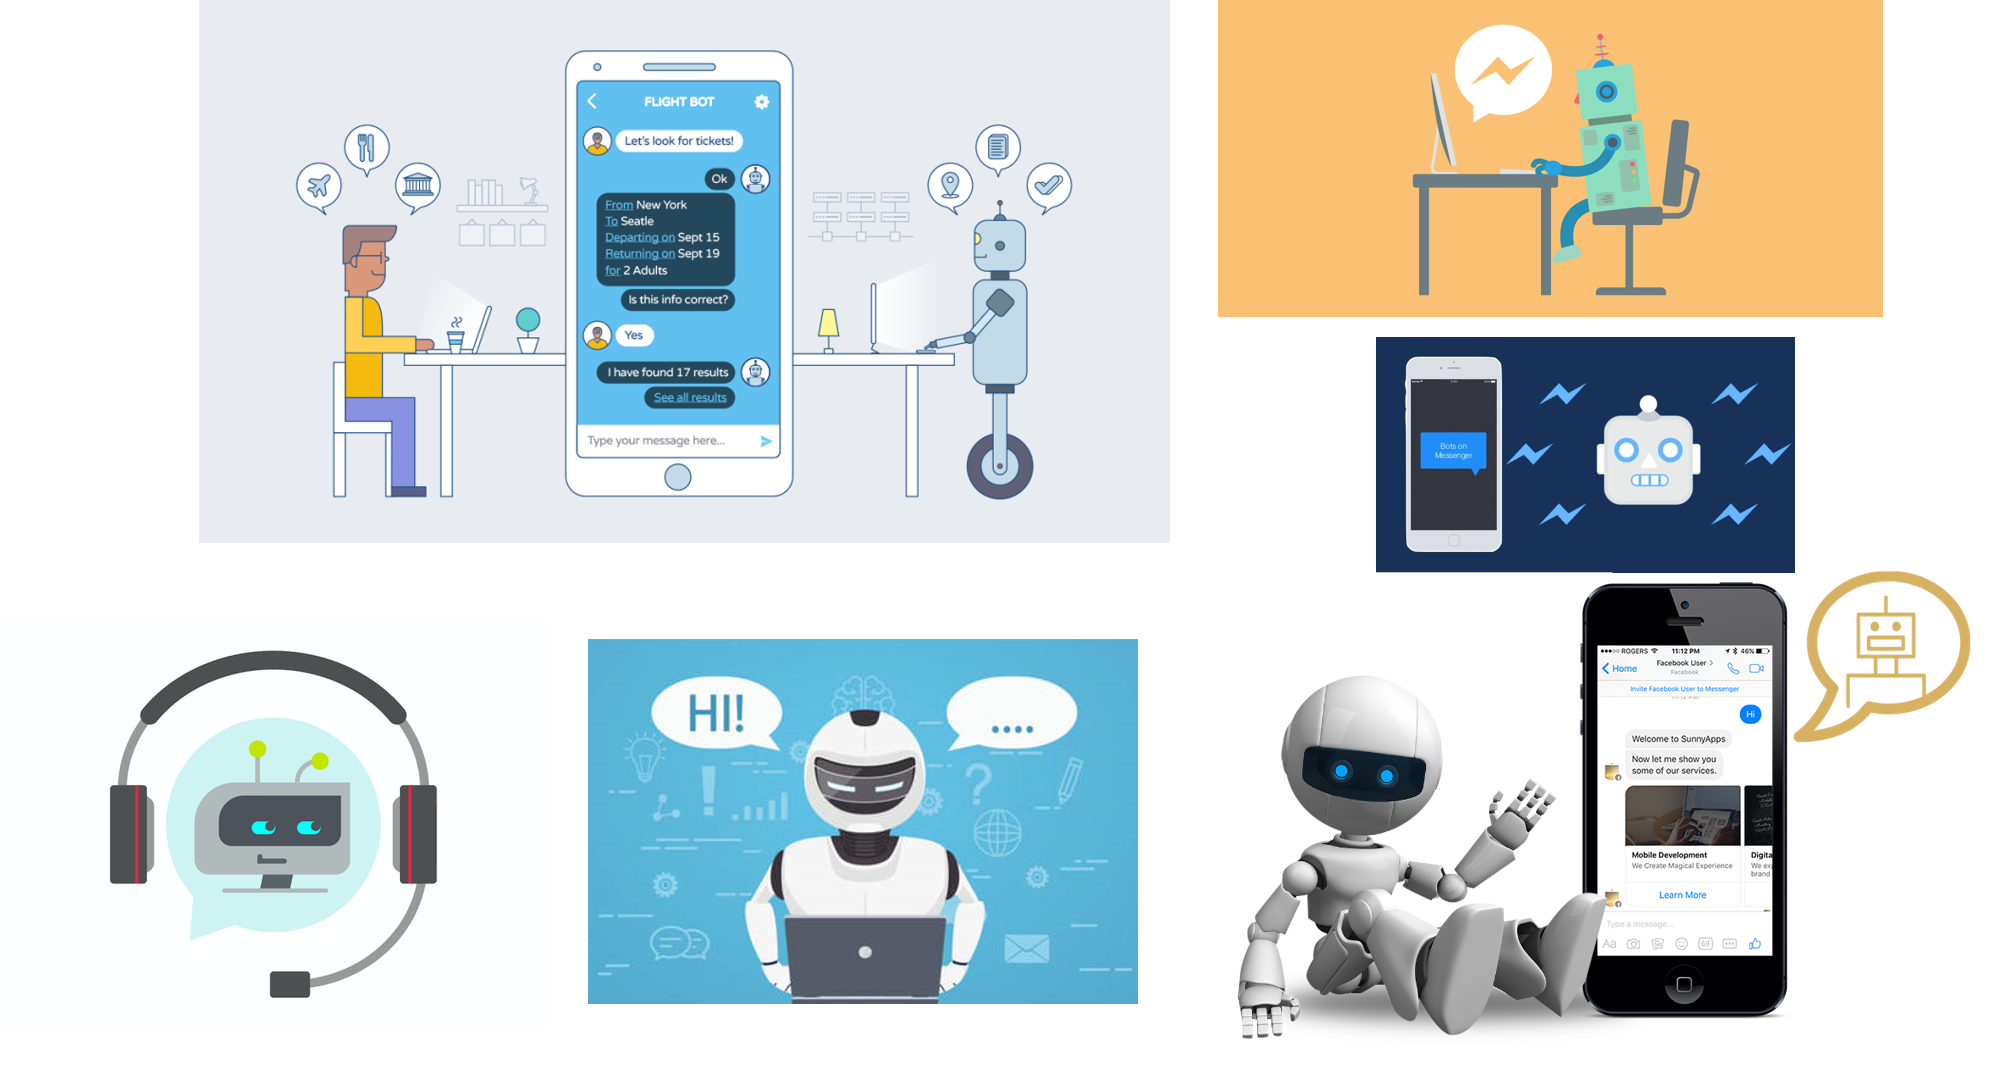
\includegraphics[scale=.5]{face}
\caption{Ref 1}
\end{center}
\end{figure}
\noindent Recently, there have been major increase of interest in use and deployment of dialogue generation systems. Many major tech companies are using virtual assistant or chat agent to fill the needs of customers. Some of them include Google's Google Assistant, Microsoft's Cortana and Amazon's Alexa. Though they are primarily question answering systems, their adoption by major corporations has peaked interest in customers and seems promising for more advanced conversational agent system research and development.\\

{\let\clearpage\relax \chapter {Related Works}}
\noindent There have been many recent development and experimentation in conversational agent system. Apart from traditional chatbot development techniques that use rule based techniques, or simple machine learning algorithms, many advanced chatbots are using advanced Natural Language Processing (NLP) techniques and Deep Learning Techniques like Deep Neural Network (DNN) and Deep Reinforcement Learning (DRL).
\section{Sequence to Sequence (Seq2Seq)}
Some of the state of the art techniques involve using Deep Neural Network and it's architectural variations. Sequence to Sequence (Seq2Seq) model based on encoder-decoder architecture is such an architecture which is very popular for dialogue generation, language modeling and machine translation. Seq2Seq uses Recurrent Neural Network(RNN) which is a popular Deep Neural Network architecture specially for Natural Language Processing tasks. In Sequence to Sequence (Seq2Seq) model, many to many RNN architecture is used for decoder. In this, encoder-decoder architecture, input sequence is fed as a vector representation of text to encoder. Then, encoder produces some intermediate representation of information or thought vectors. Consequently, the thought vector generated by encoder is fed into decoder as input. Finally, decoder processes the thought vector and converts the sequence one by one word and produces multiple output from the decoder in form of target sequence. Though, vanilla RNN is default in Seq2Seq and works well for many NLP problems yet, due to higher complexity of language modeling problem, vanilla recurrent neural network cells often fails, specially, where long sequence of information needs to be remembered, as this information frequently becomes large for bigger datasets and turns to information bottleneck for the RNN network. Therefore, researchers uses variations of recurrent neural network to handle such problem.
\begin{figure}[H]
\begin{center}
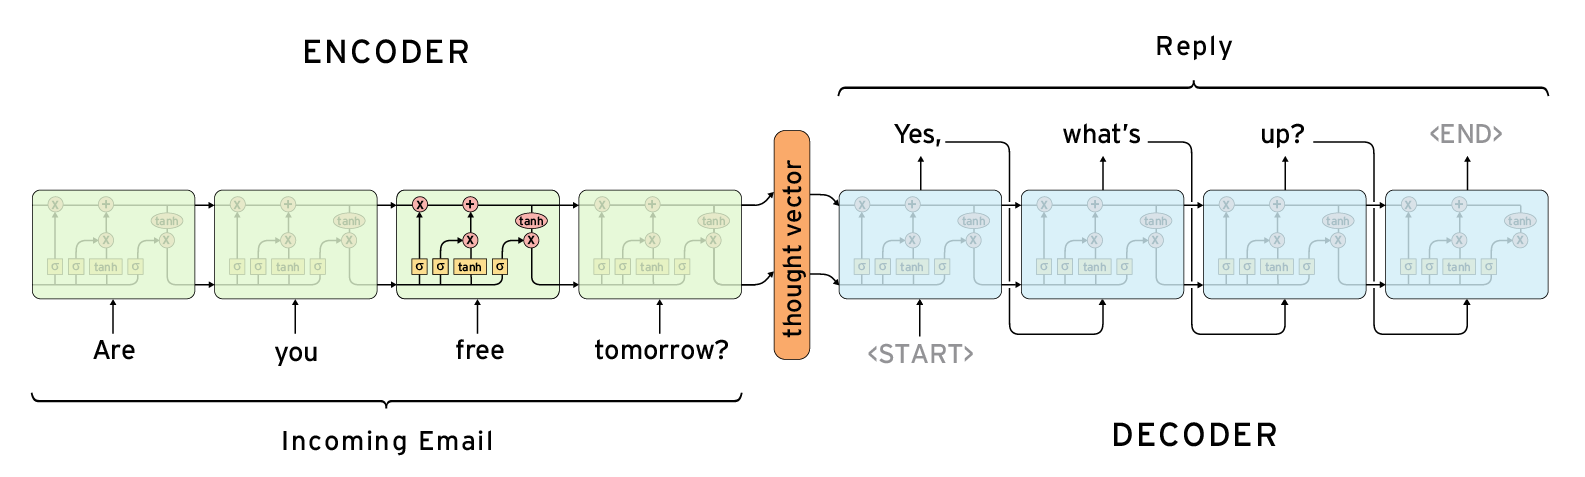
\includegraphics[scale=.3]{seq2seq_related}
\caption{Sequence to Sequence Model}
\end{center}
\end{figure} 
\noindent Long-Short-Term-Memory(LSTM) is a special variant of cell type of Recurrent Neural Network which has empirically shown to work well for language modeling. LSTM has forget gates along with input gates and output gates. This helps remember more relevant and contextual information and discards the rest of the sequence which is desirable in language modeling where dependency within sequence is sparse. Also, instead of using unidirectional cells, bidirectional LSTM cells can perform much better.\\\\
Another technique, Neural Attention Mechanism embedded in Seq2Seq module has significantly improved performance in dialogue generation system and other NLP tasks and thus become industry standard practice. In Neural attention mechanism, each hidden target compares with source hidden state, generates attention vector by calculating score and preserves the attention vector in memory to choose over other candidate. Also, other techniques like, Beam Search can help improve decoding performance further by choosing top candidates. Seq2Seq have also been applied for other NLP tasks including machine translation, text summarization and question-answering and image captioning.
\begin{figure}[H]
\begin{center}
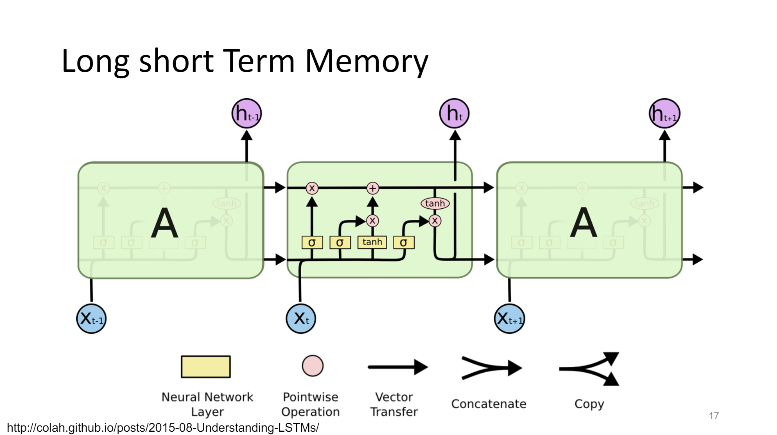
\includegraphics[scale=.4]{lstm}
\caption{Ref 7}
\end{center}
\end{figure} 
\section{Google's Neural Machine Translation(GNMT)}
Google's Neural Machine Translation(GNMT) model is a module for neural machine translation from and to other language and English. GNMT has also been used for dialogue generation experimentally. It is based on Seq2Seq model which is popular in dialogue generation. Also, GNMT has many techniques embedded in the module which are crucial for intelligent chatbot development. The GNMT model includes, Sequence to Sequence modeling with encoder-decoder architecture built using uni or bi directional LSTM cells. They also have option for Neural Attention Mechanism, Beam Search, and vocabulary generation using Google's sub-word module. Also, they have option for adjusting the hyper-parameters for better model training.
\section{Deep Reinforcement Learning}
"Deep Reinforcement Learning for Dialogue Generation"\cite{jurafskyRL} of  Dan Jurafsky, Deep Reinforcement Learning (DRL) has been used for developing long conversation chatbots. Seq2Seq model can generate coherent dialogues but may produce repeated generic responses regardless of input and can get stuck in a loop in longer conversations. This occurs as Seq2Seq predicts utterances one at a time while ignoring their influence on future outcomes. Seq2Seq models tend to generate highly frequent repeated responses like  "I don't know". This is due to high frequency of generic responses in the training set, also this replies are more compatible with a wide range of input text.
\begin{figure}[H]
\begin{center}
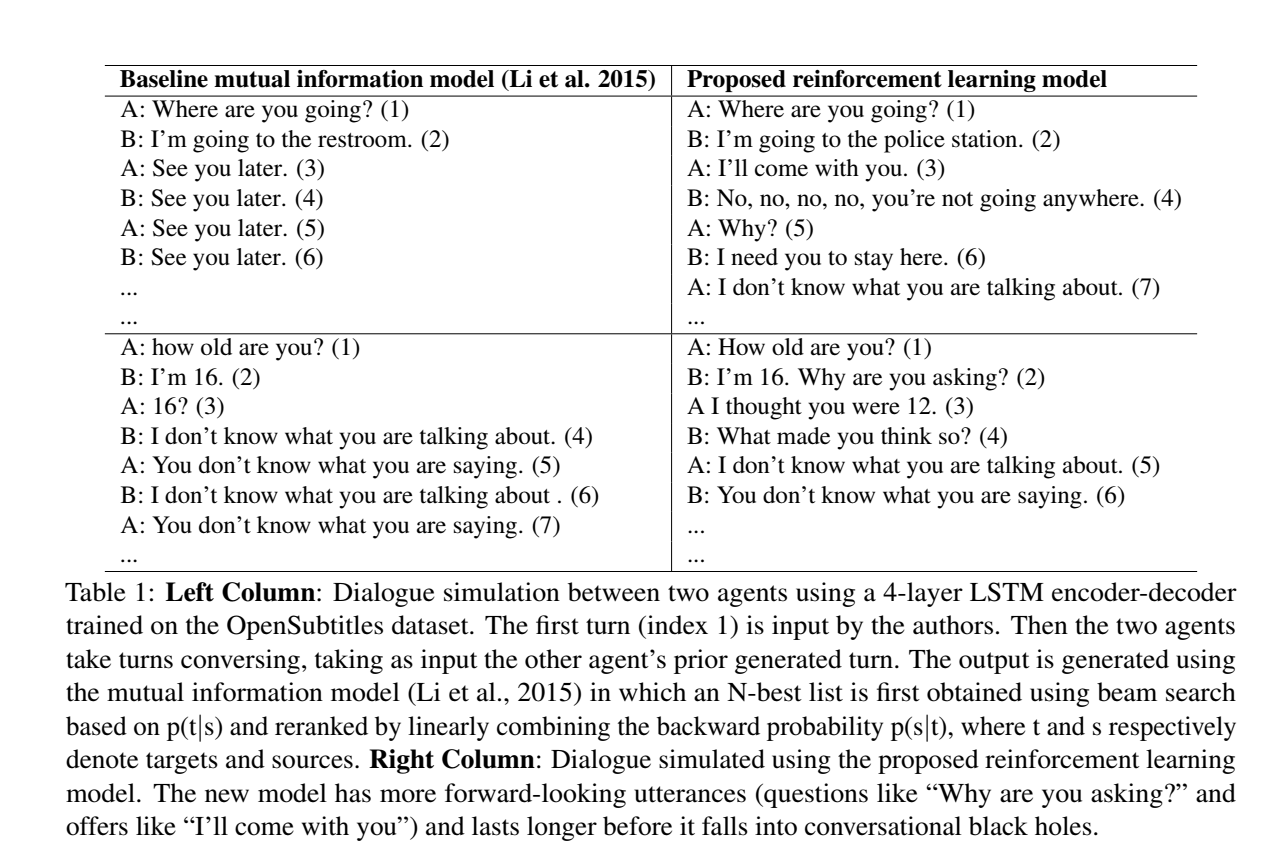
\includegraphics[scale=.5]{DRL1}
\end{center}
\end{figure} 
\noindent In Dufarsky's paper, they have generated intermediate response using Seq2Seq model with attention where input was raw text. Then, the intermediate generated responses were fed into Reinforcement Model and was rewarded based on Ease of answering, Information Flow and Semantic Coherence. This is forward centric model, where if generated response is easy to answer, contribute to more information compared to previous dialogue history and grammatically and semantically correct, they are rewarded.
\begin{figure}[H]
\begin{center}
%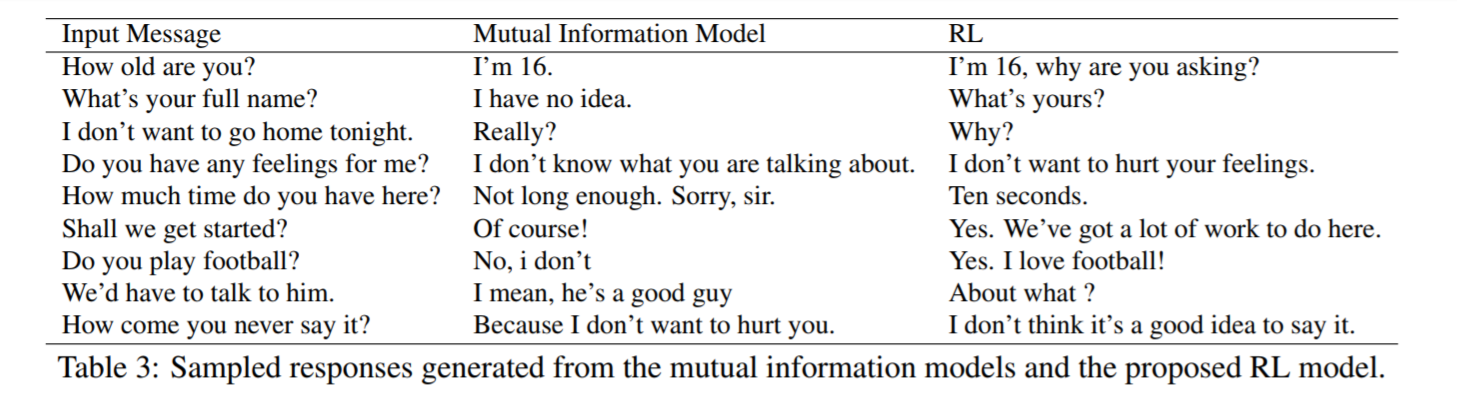
\includegraphics[width=15cm, height=5cm]{chatbot_research_conv1}
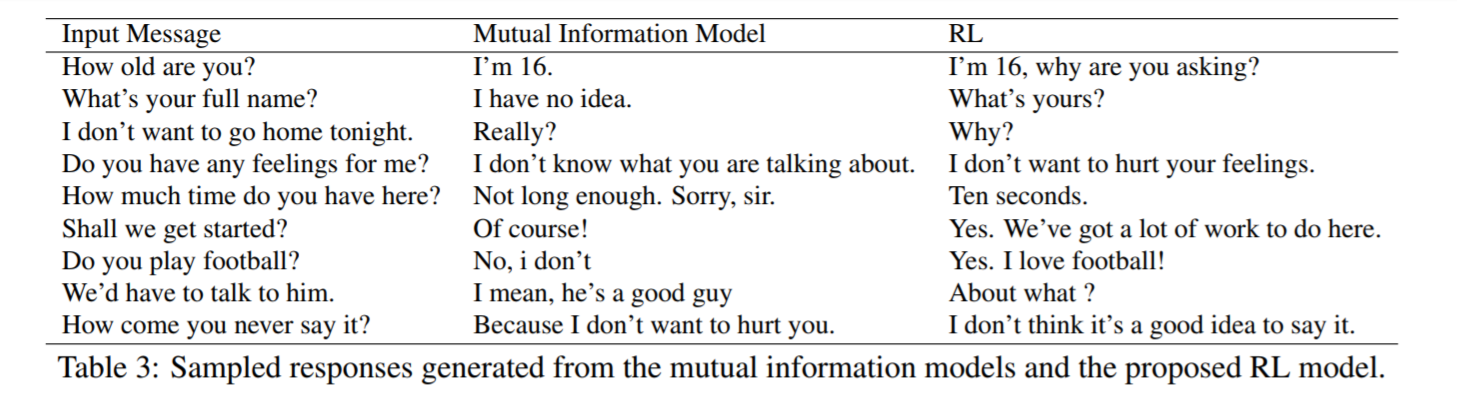
\includegraphics[scale=0.33]{chatbot_research_conv1}
\end{center}
\end{figure}
\noindent Despite success, in this paper Dufarsky has stated that the RL model is not optimized to predict the next utterance. This model increased long-term reward for longer conversation to keep conversation going by reducing generic response. But, less relevant responses are produced in their experimentation as there is trade-off between relevance and less repetitiveness.
\newpage
{\let\clearpage\relax \chapter {Limitations}}
\noindent Although, there are many chatbots currently available, majority of them are limited in functionality, domain function, context and coherence. They often fail in long conversations and have reduced relevancy in dialogue generation. Most of these chatbots are developed for restricted domain. Majority of them are using simple rule based techniques. They perform well in question answering sessions and in very structured conversational modes. But, fail to emulate real human conversation and lacks flexibility in functioning. Some of the chatbots using machine learning algorithms often adhere to simple algorithms. They lack in complexity and sophistication needed to produce good result specifically in open domain conversation.\\\\
Some chat engines are available in market which are often used by businesses for developing automated customer support. They are also black box and business clients have limited knowledge of their internal architectures. Hence, they produce results that can become unreliable and fail to fill the need of customers.
Following is an example of failed chatbot replies.
\begin{figure}[H]
\caption{Some undesirable chatbot replies (ref 5)}
\begin{center}
\begin{minipage}{0.49\textwidth}
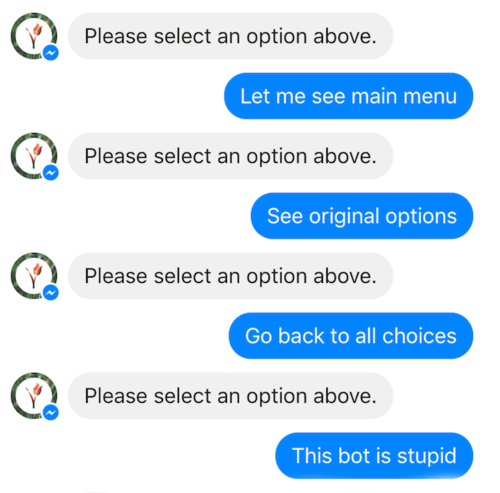
\includegraphics[scale=.4]{chatbotfail1}
\end{minipage}
\begin{minipage}{0.49\textwidth}
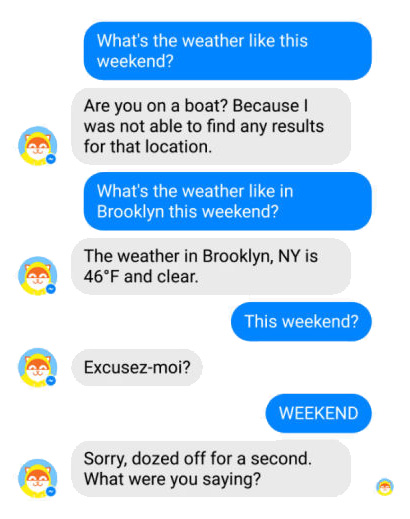
\includegraphics[scale=.45]{chatbotfail2}
\end{minipage}
\end{center}
\end{figure}
\newpage
{\let\clearpage\relax \chapter {Deep Neural Network for Chatbot}}
\section {Recurrent Neural Network}
Recurrent Neural Network is a special Deep Neural Network Architecture used predominantly in Natural Language Processing (NLP) problems. In traditional Deep Neural Network, memory or sequence information is not taken into account. But, in Recurrent Neural Network, the sequential information is stored in memory and utilized for further processing which makes RNN suitable for sequential data or time series data where dependency exists in sequence.
\subsection {Recurrent Neural Network Architecture}
Recurrent Neural Network (RNN) is composed of input layer, multiple hidden layers and output layer. In input layer, input is feed as vector representation. Then, input vector is multiplied by some weight and some biases are added. Then, the output from input layer is passed to next hidden layer where each consecutive hidden layer is composed of numerous RNN cells. After getting output from input layer, the cells in hidden layer multiplies the generated output from input layer by their own cell weights and biases. Next, in each of the hidden layer cells, some global activation function (sigmoid, tangent) is applied to generate output from hidden layer. Then, output from each hidden layer cells is passed to successive hidden layer. Similar to previous hidden layer cells, some weight, biases and activation function is applied to the input of current hidden layer cell. This procedure propagates though all consequent hidden layers. Finally, output generated from the final hidden layer is passed to output layer and the output layer applies some function (e.g. Softmax) to generate final output. For RNN, the output vector from final output layer is then again fed into the input layer as an input vector. Hence, the sequence information is stored in the memory and utilized. 
\begin{figure}[H]
\begin{center}
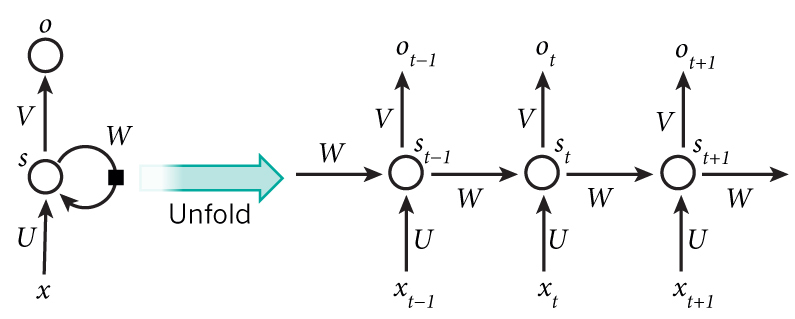
\includegraphics[scale=.25]{rnn1}
\caption{Recurrent Neural Network}
\end{center}
\end{figure}
\noindent But, vanilla RNN stores the complete sequence information. For large dataset with longer sequences, this can cause information bottleneck for the network. It may cause network to perform poorly due to information overload. As in many cases, complete sequential information may not be relevant in many NLP task including dialogue generation and can cause model to perform poorly. This problem is solved by special type of RNN cell Long-Short-Term-Memory(LSTM).
\subsection {Long-Short-Term-Memory(LSTM)}
Long-Short-Term-Memory(LSTM) is a special type of Recurrent Neural Network cell, which solves the data bottleneck for longer sequences. LSTM has forget gate along with the input and output gates. This helps remember longer sequence without overloading the network by discarding less relevant information.
\begin{figure}[H]
\begin{center}
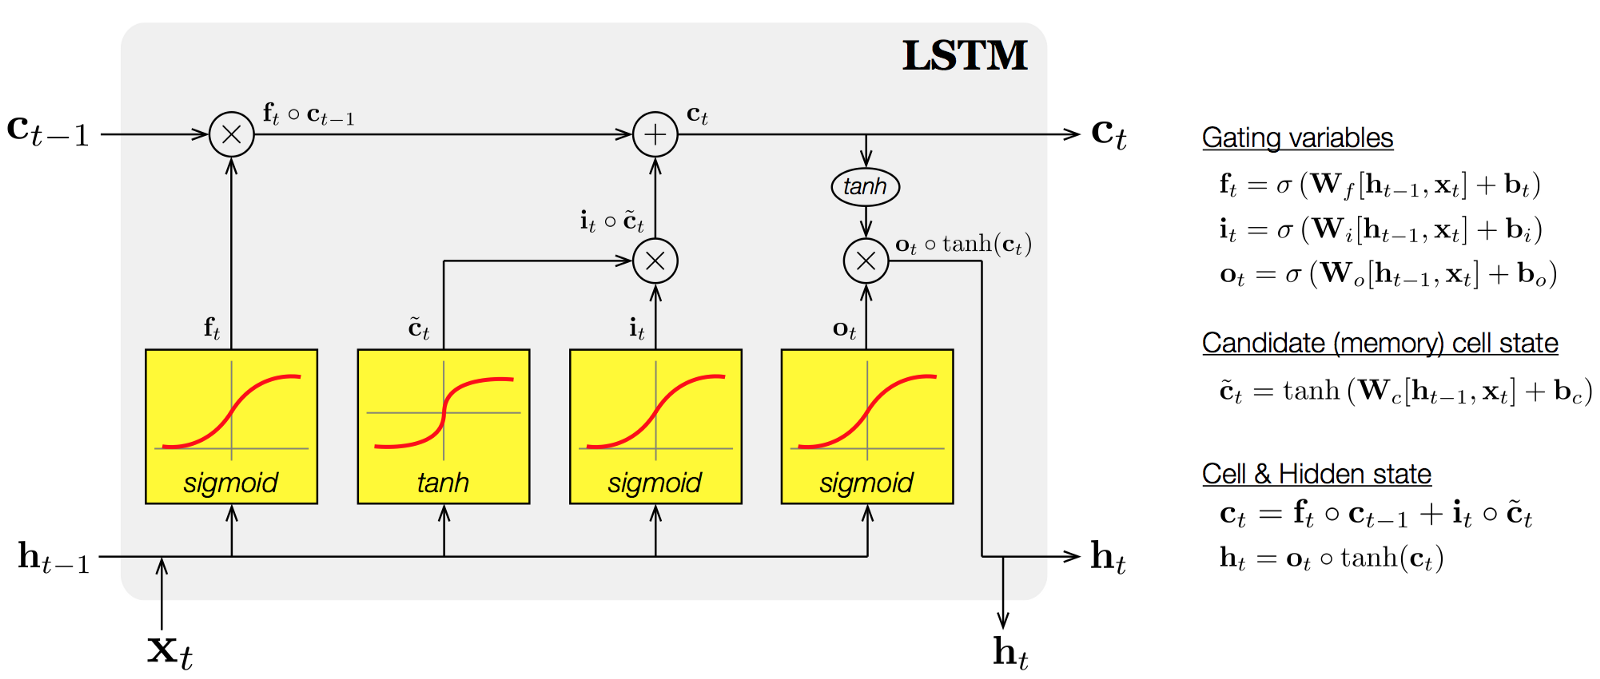
\includegraphics[scale=.22]{lstm2}
\caption{Long-Short-Term-Memory(LSTM)}
\end{center}
\end{figure}
\noindent There are couple of variation of LSTM. Following is the equation for LSTM with forget gate.\\\\
$f_t = \sigma_g(W_fx_t+ U_fh_{t-1}+b_f)$\\
$i_t = \sigma_g(W_ix_t+ U_ih_{t-1}+b_i)$\\
$o_t = \sigma_g(W_ox_t+ U_oh_{t-1}+b_o)$\\\\
$c_t = f_t . c_{t-1} +i_t.\sigma_g( \sigma_g(W_cx_t+ U_ch_{t-1}+b_c)$\\
$h_t = o_t . \sigma_h(c_t)$\\\\
\textbf{Variables}\\\\
$x_{t}\in R^{d} : \text{ input vector to the LSTM unit}$\\
$f_{t}\in R^{h} : \text{ forget gate's activation vector}$\\
$i_{t}\in R^{h} : \text{ input gate's activation vector}$\\
$o_{t}\in R^{h} : \text{ output gate's activation vector}$\\
$h_{t}\in R^{h} : \text{ output vector of the LSTM unit}$\\
$c_{t}\in R^{h} : \text{ cell state vector}$\\\\
$W\in R^{h\times d}, U\in R^{h\times h} \quad and \quad b\in R^{h} :$ weight matrices and bias vector parameters which need to be learned during training where the superscripts d and h refer to the number of input features and number of hidden units, respectively.\\\\
\textbf{Activation functions}\\\\
$\sigma _{g} : \text{ sigmoid function.}$\\
$\sigma_c : \text{ hyperbolic tangent function.}$\\
$\sigma _{h} : \text{ hyperbolic tangent function,} \sigma _{h}(x)=x$.\\\\

{\let\clearpage\relax \chapter {Architecture}}
\noindent In this project, I have developed Intelligent conversational agent following state of the art techniques proposed in recently published research papers. I have used Google's Neural Machine Translation(GNMT) module for building dialogue generator. Although, Google's Neural Machine Translation(GNMT) module is primarily used for Machine Translation tasks, they have empirically shown to be successful in other NLP tasks including dialogue generation and text summerization. GNMT has rich Seq2Seq module with many additional features for dialouge generation. Seq2Seq is a industry standard choice for dialogue generation and many NLP tasks. Althought, there exists a separate Seq2Seq module\cite{seq2seq} which was the the early robust Seq2Seq module, but is not currently compatible with latest version of Google's machine learning framework Tensorflow and is only compatible with Tensorflow v1.0 whereas current Tensorflow is v1.6. Also, earlier version of Tensorflow had a minimalistic Seq2Seq module, it is not efficient for building robust model. Currently, Google does not offer any robust Seq2Seq module in it's official Machine Learning Framework Tensorflow and has moved many functionality of Seq2Seq to NMT model. Moreover, GNMT has many techniques embedded for dialogue generation agent development. GNMT model includes, Sequence to Sequence modeling (Seq2Seq) with encoder-decoder architecture based on uni or bi directional LSTM cells. GNMT also have option for Neural Attention Mechanism, Beam Search, and vocabulary generation using Google's sub-word module.\\
\section {Google's Neural Machine Translation (GNMT)}
\subsection {Sequence to Sequence (Seq2Seq) Architecture}
Google's Neural Machine Translation (GNMT) is primarily used for machine translation. But, GNMT contains Sequence to sequence module with many enhancement techniques which can help build good dialogue generator. For translation, GNMT, does not apply traditional phrase-based translation systems where translation is performed by breaking up source sentences into multiple chunks and then translate phrase-by-phrase. It rather uses more human like translation approach. 
\begin{figure}[H]
\begin{center}
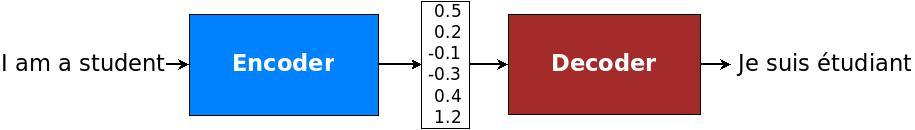
\includegraphics[scale=.5]{encdec}
\caption{Encoder-decoder architecture – example of a general approach for NMT. An encoder converts a source sentence into a "meaning" vector which is passed through a decoder to produce a translation.}
\end{center}
\end{figure}
\noindent GNMT is based on Seq2Seq architecture composed of encoder-decoder unit. GNMT can be used with with different variation of architectures. The Seq2Seq module is composed of encoder and decoder. Encoder takes source text as input and processes the text to generate intermediate representation of input text called thought vector. The thought vector is then fed into the decoder input unit. The decoder now processes the thought vector and generates outputs. In case of dialogue generation problem the output is a response and for machine translation problem output is the target text. This architecture have shown to be capable of processing long-range dependencies and produce more fluent translations or responses.\\\\
Encoder-decoder units of GNMT's Seq2Seq module can have different architectures. Both encoder and decoder is composed of Recurrent Neural Network (RNN). But RNN of encoder and decoder unit can be composed of different cell types other than vanilla RNN cell, including Long Short-term Memory (LSTM), or a gated recurrent unit (GRU). Also, encoder and decoder can be composed of unidirectional or bidirectional RNN. But, it has been empirically found that, LSTM works well for dialogue generation and other language problems as full sequence text can become information bottleneck and in many cases complete sequence is not required for efficient dialogue generation. Also, bidirectional RNN can help improve performance further more. In my project I have used GNMT module with bidirectional LSTM cell. The architecture of this project consists of 2 layer encoder-decoder unit with 512 units.
\begin{figure}[H]
\begin{center}
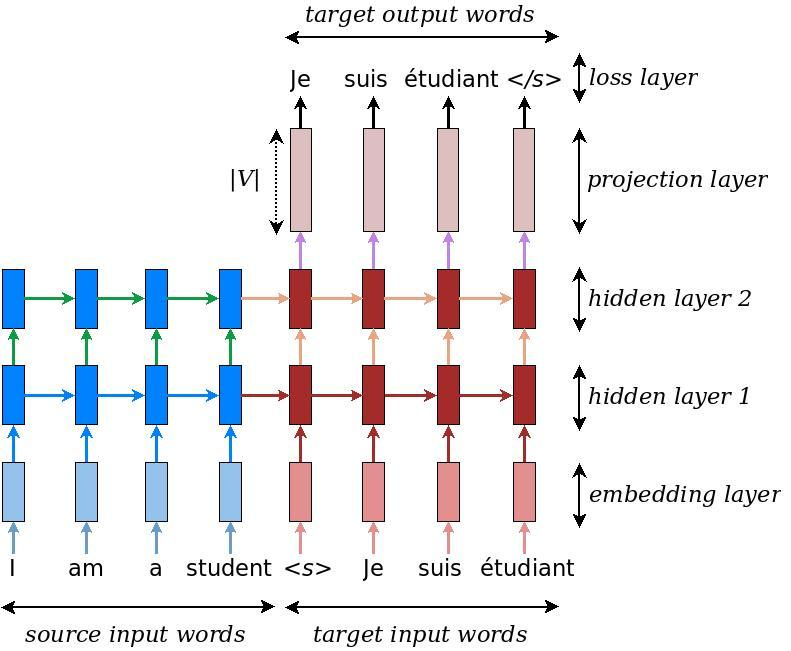
\includegraphics[scale=.35]{seq2seq}
\caption{Neural machine translation – example of a deep recurrent architecture proposed by for translating a source sentence "I am a student" into a target sentence "Je suis étudiant". Here, "$<s>$" marks the start of the decoding process while "$</s>$" tells the decoder to stop.}
\end{center}
\end{figure}
\newpage
\subsubsection {Neural Attention Mechanism\cite{nmt}}
To build state-of-the-art neural machine translation systems, the attention mechanism works specially well, which was first introduced in 2015. The idea of the attention mechanism is to form direct short-cut connections between the target and the source by paying "attention" to relevant source content as we translate\cite{nmt}.
\begin{figure}[H]
\begin{center}
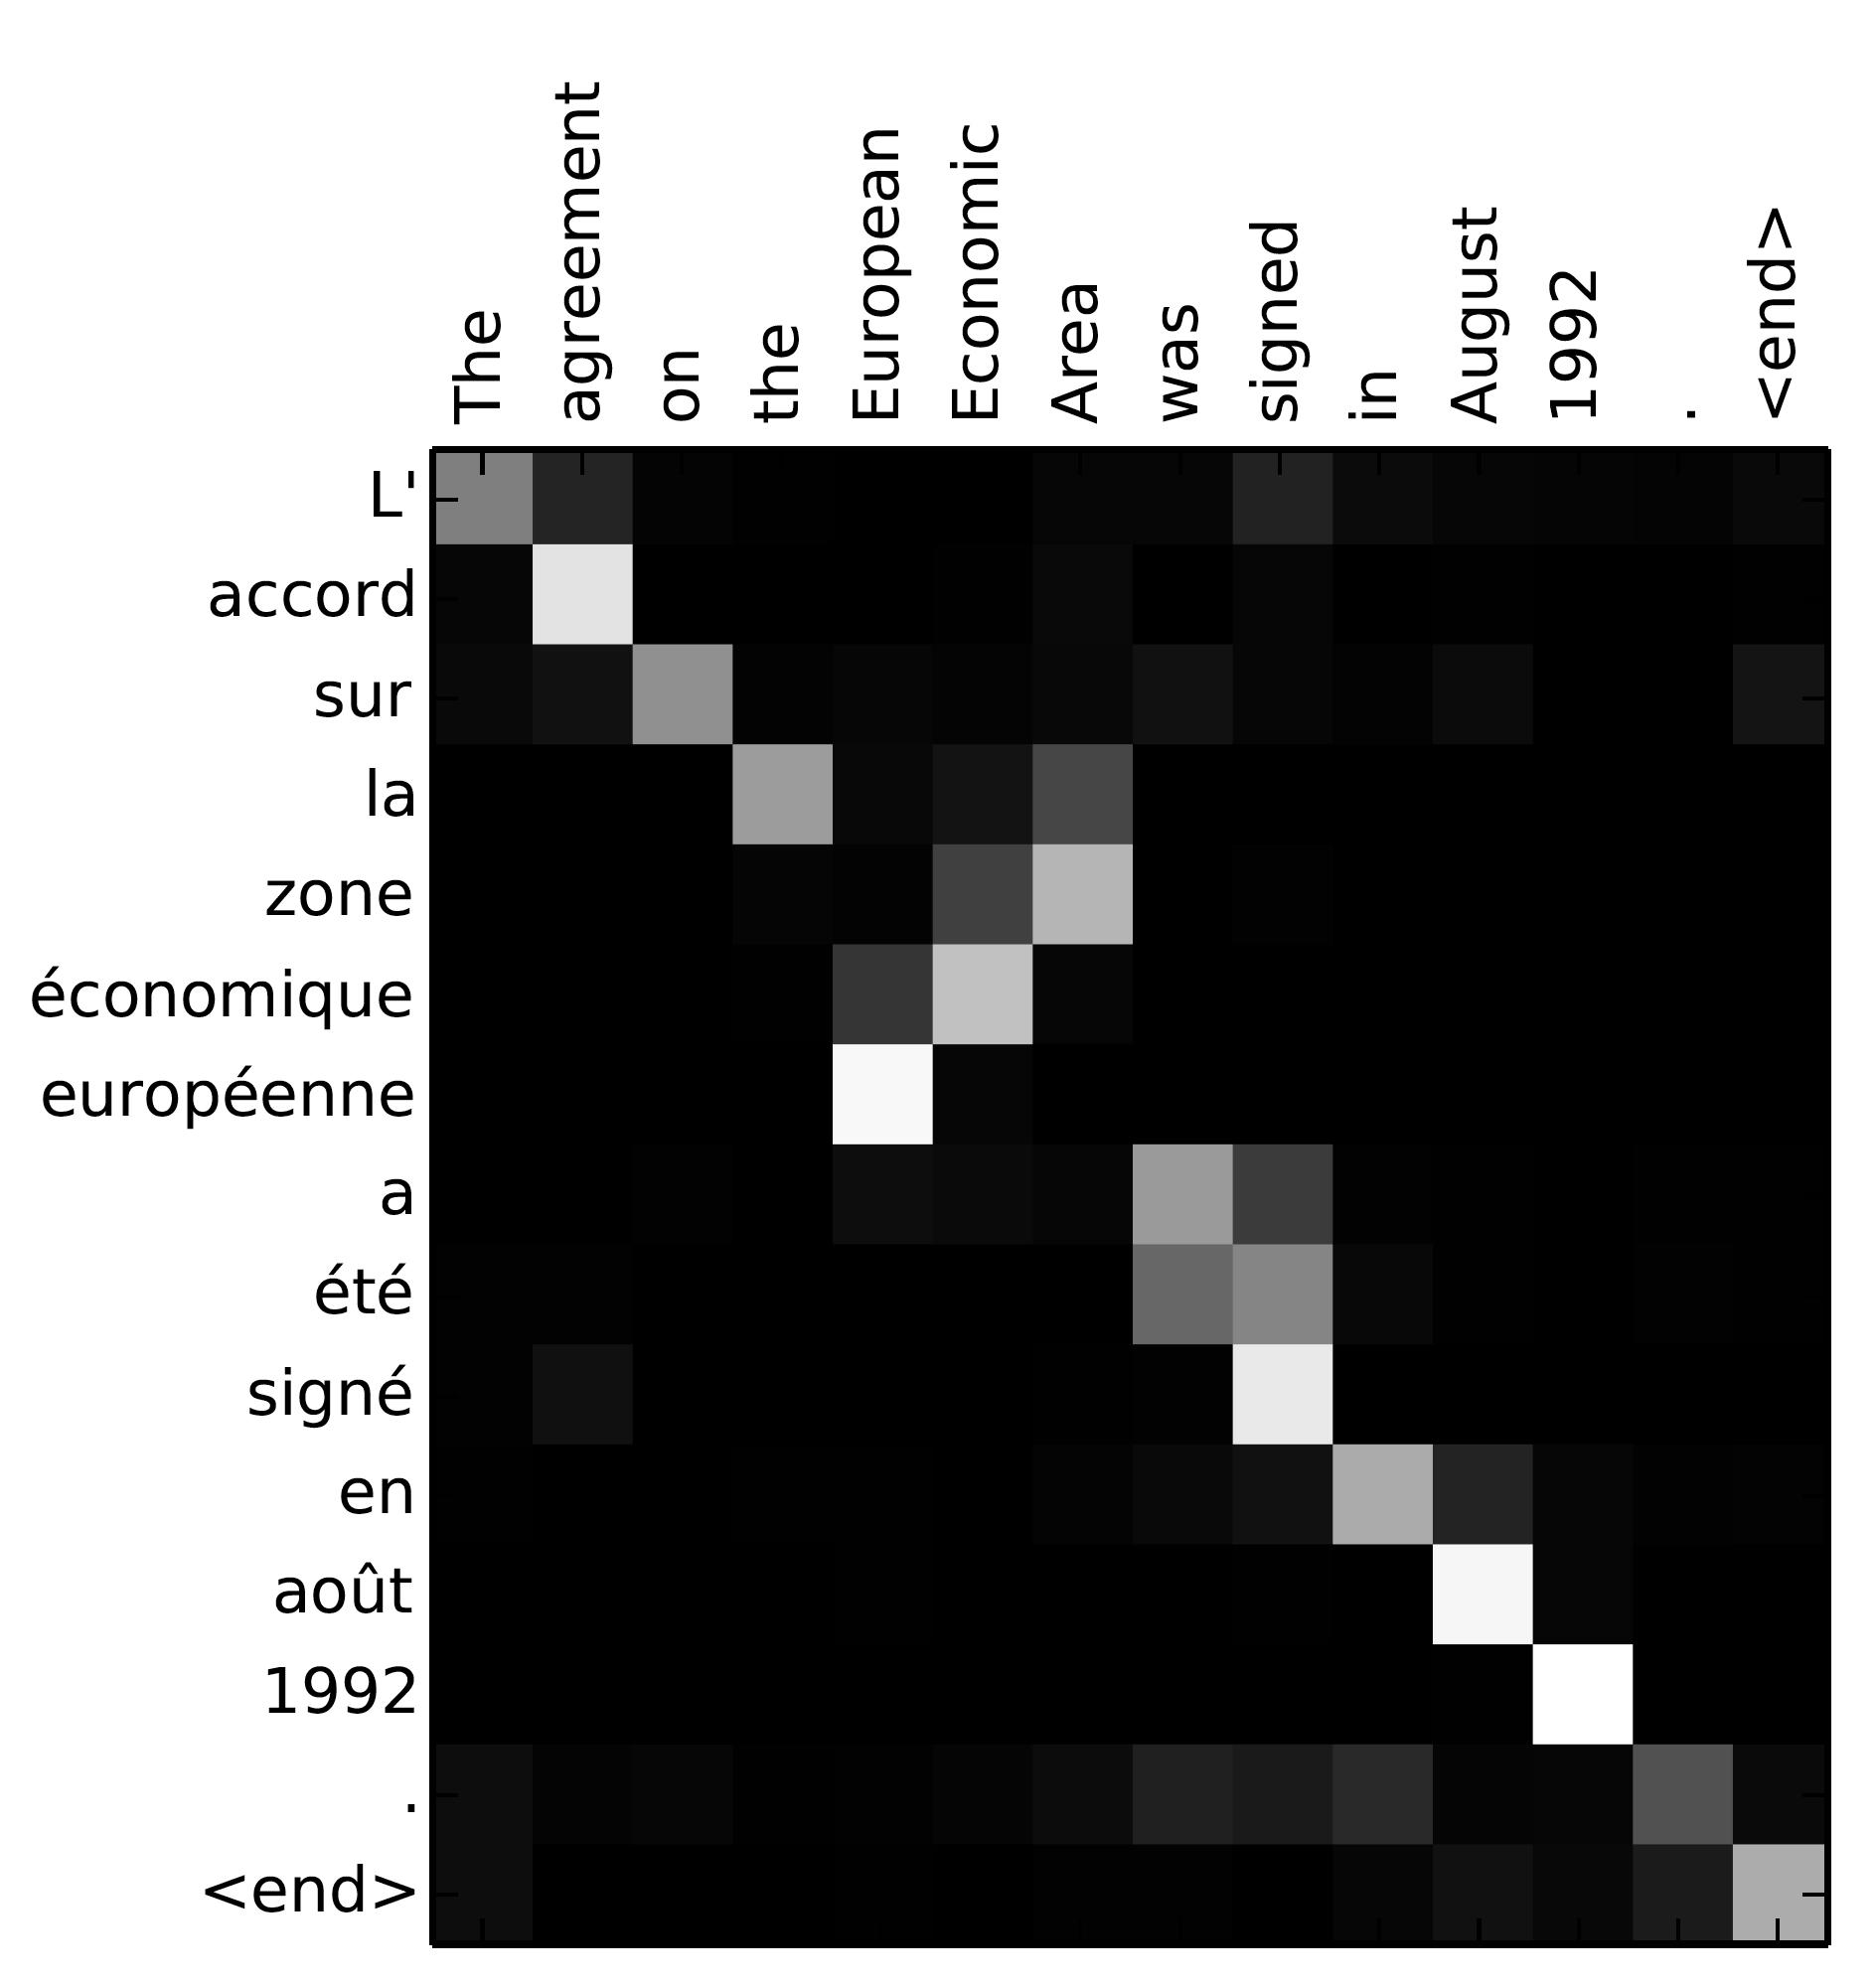
\includegraphics[scale=.1]{attention_vis}
\caption{Attention visualization – example of the alignments between source and target sentences}
\end{center}
\end{figure}
\noindent In the vanilla seq2seq model, the last source state from the encoder to the decoder is passed when starting the decoding process. This works well for short and medium-length text string. However, for long sentences, the single fixed-size hidden state becomes an information bottleneck. Instead of discarding all of the hidden states computed in the source RNN, the attention mechanism provides an approach that allows the decoder to peek at them (treating them as a dynamic memory of the source information). This attention mechanism improves the translation of longer sentences. Attention mechanisms are the industry standard and applied to  other NLP tasks including image caption generation, speech recognition, and text summarization.
\begin{figure}[H]
\begin{center}
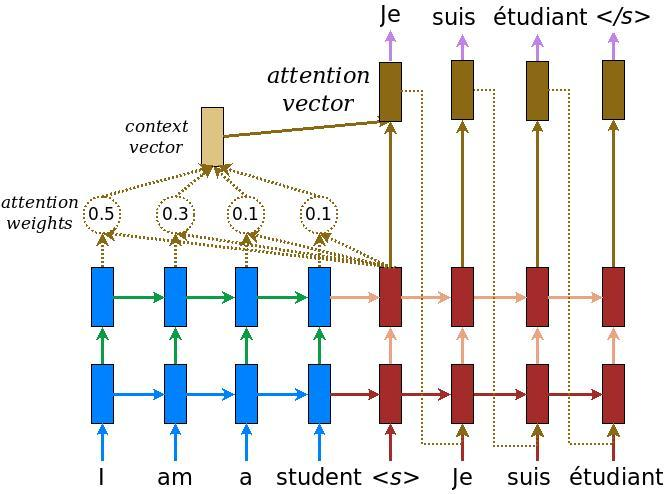
\includegraphics[scale=.3]{attention_mechanism}
\caption{ Attention mechanism – example of an attention-based NMT system.}
\end{center}
\end{figure}
\noindent As illustrated in Figure 5.4, the attention computation happens at every decoder time step. It consists of the following stages:
\begin{enumerate}
\item The current target hidden state is compared with all source states to derive attention weights
\item Based on the attention weights we compute a context vector as the weighted average of the source states.
\item Combine the context vector with the current target hidden state to yield the final attention vector.
\item The attention vector is fed as an input to the next time step. The first three steps can be summarized by the equations below:
\begin{align*}
a_{ts} = \frac{exp(score(h_t, \bar{h_s}))}{\sum_{s'=1}^{S}{exp(score(h_t, \bar{h_{s'}}))}} \qquad\text{[Attention weights]}\qquad(1)\\
c_t = \sum_{s}^{}{a_{ts}\bar{h_s}} \qquad\text{[Context vector]}\qquad(2)\\
a_t = f(c_t, h_t) = tanh(W_c[c_t,h_t]) \qquad\text{[Attention vector]}\qquad(3)
\end{align*}
\end{enumerate}
\begin{figure}[H]
\begin{center}
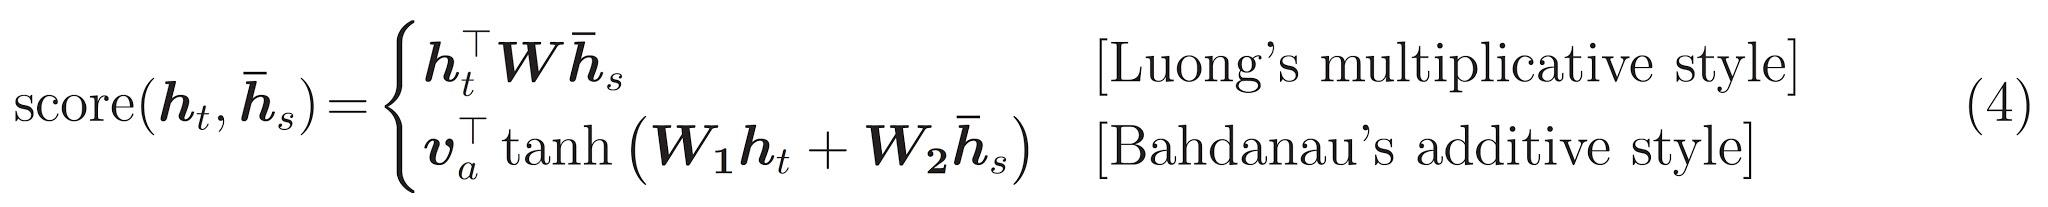
\includegraphics[scale=.18]{attention_equation_1}
\end{center}
\end{figure}
Here, score function is used to compare the target hidden state "$h_t$" with each of the source hidden states "$\overline{h}_s$". The result is then normalized to produce attention weights which is a distribution over source positions. There are different choices for score function including multiplicative and additive forms. Once computed, the attention vector "$a_t$" is used to derive the softmax logit and loss.\\\\

{\let\clearpage\relax \chapter {Data}}
\section {Data Collection}
In this project, the dataset "Cornell Movie Subtitle Corpus" has been primarily used for final model training. Few other dialogue corpus based on movie subtitles have been preprocessed and cleaned for GNMT training including "Open Movie Subtitle Corpus" and "Movie Subtitle Corpus". But due to lack of data quality, they have been eliminated from final training.\\\\
For future work, more robust and real life conversation based corpus can be incorporated for dialogue generation model building if available. Other possible candidates for dialogue corpus includes, twitter data, reddit dataset and relay chat engine data corpus.
\subsection {Dataset 1: Cornell Movie Subtitle Corpus}
For developing final chatbot, popular movie subtitle corpus "Cornell movie subtitle corpus" has been used. This corpus contains metadata-rich large collection of conversations extracted from raw movie scripts from popular movies.\\
The following are found in corpus-
\begin{itemize}
\item[-] 220,579 conversational exchanges between 10,292 pairs of movie characters.
\item[-] involves 9,035 characters from 617 movies
\item[-] in total 304,713 utterances
\end{itemize}
Other movie meta-data included genres, release year, IMDB rating, number of IMDB votes, IMDB rating\\\\
The data corpus can be found in \url{http://www.cs.cornell.edu/~cristian/Cornell_Movie-Dialogs_Corpus.html}.
\section {Data Preprocessing}
Data was processed to prepare for input pipe line of the Google's Neural Machine Translation(GNMT) model. In the original GNMT model, there were two input data files and two vocabulary file generated from input files. The two input files were translation from and translation to language input data file. The vocabulary files contained the processed vocabulary for the two input data file of two different language respectably. Also, there were separate test and development file for source and target.
\subsection {Preprocessing of Cornell Movie Subtitle Corpus}
Conversation data in the movie corpus contained Movie ID, Character ID, and Movie Line ID was separated by "+++++".\\\\
For preprocessing, conversation data was cleaned to remove these meta-data(eg. movie ID, character ID, Line ID). Also, data separators("+++++") were eliminated. Additionally, some of the character in the data contained unsupported encoding format by UTF-8 standard and was hence removed.\\\\
Finally, data was separated in two different files to assimilate with the format of Google's Neural Machine Translation(GNMT) model input pipeline format where first file is the dialogue 1 and second one was response to dialogue 1.\\\\
After separating the two files, data in both file was cleaned simultaneously. Everything except alphabetical character, and some punctuation (. , ?!') was removed as they hold little meaning in conversation. Also, all the text was converted to lowercase. Then, multiple consequent occurrence of these punctuation (. , ?!') was reduced to one in order to reduce punctuation overload. Next, all the punctuation except (') was separated with single space before and after for better performance in GNMT module. Finally, all the consequent multiple space was reduced to single space and each text string was trimmed to remove before and after space.\\\\
Also, data was cleaned for removing extraneous dialogues. If multiple consequent utterance from single person was present everything except the last utterance for the person was stored. Initially, utterance with more than 100 length was discarded for both text dialogue and their reply as with increase of length the text, context relevance starts to drop due to diversity and limited data. But later full text length was embedded.\\\\
After through clenaing, the source and target text was splitted for training, testing and development/validation set with source and target format and was saved in files for final input pipeline feed.\\\\
For vocabulary generation, Google's Sub-word Neural Machine Translation(NMT) module was used as suggested by the Google Tensorflow and Google's Neural Machine Translation module documentation. The sub-word application was only applied on training files source and target files.\\\\

{\let\clearpage\relax \chapter {Implementation Summary}}
\begin{center}
\begin{table}[H]
\caption{Algorithm Details}
\bigskip
\begin{tabular}{|lll|}
\hline
Deep Learning Module & : & Google's Neural Machine Translation (NMT).\\ 
Algorithm &:& Deep Neural Network (DNN), Recurrent Neural Network (RNN)\\
Main Technique&:&Sequence to Sequence (Seq2seq) modeling \\
&&with encoder and decoder\\
Enhancement Techniques &:& Long Short Term Memory (LSTM) based RNN cell,\\
&&Bidirectional LSTM, Neural Attention Model and Beam Search.\\
\hline
\end{tabular}
\end{table}
\end{center}
\vspace{-3em}
\begin{table}[H]
\caption{Front-end and Back-end}
\bigskip
\begin{center}
\begin{tabular}{|lll|}
\hline
Front-end &:& Python with PyQT.\\
Back-end &:& Python.\\
\hline
\end{tabular}
\end{center}
\end{table}
\newpage
{\let\clearpage\relax \chapter {Hardware Specification}}
\noindent For training, personal laptop with 7th Gen Intel Core i5 Processor,  dedicated graphics-NVIDIA GTX 1050 and 8GB Ram has been used. For further extended training, cloud computing platform Amazon AWS can be deployed. 
\begin{table}[!ht]
\caption{Hardware Platform- Local machines (personal laptop)}
\begin{center}
\begin{tabular}{|lll|}
\hline
Processor & : & 7th Gen Intel Core i5-7300HQ mobile processor.\\
Ram & : & 8GB.\\
Graphics Card & : & NVIDIA GTX 1050 graphics.\\
\hline
\end{tabular}
\end{center}
\end{table}

{\let\clearpage\relax \chapter {Experiment}}
\section {Training}
\subsection {Training Dataset}
Training has been completed on 225000*2 utterance of "Cornell movie subtitle corpus" conversation and has been tested with 5000+5000 utterance and validated with 5000+5000 utterance. 
\begin{center}
\begin{table}[H]
\begin{center}
\caption{Training Dataset}
\begin{tabular}{|l|c|c|}
\hline
Dataset (Text) & Total Number of Utterance(person 1 and person 2) & Total Size in MB\\
\hline
\hline
Training Data & 225000+225000 & 17+17\\
\hline
Testing Dataset & 5000+5000 & \\
\hline
Validation Dataset & 5000+5000 & \\
\hline
\end{tabular}
\end{center}
\end{table}
\end{center}
\subsection {Training Model and Parameters}
For training, GNMT module based on Bidirectional LSTM cells have been used. Neural Attention Mechanism have been applied to improve performance. Beam search was also applied on training but was later discarded. Total 3200 iteration with 512 hidden unit was trained with 2 layers.
\begin{figure}[H]
\begin{center}
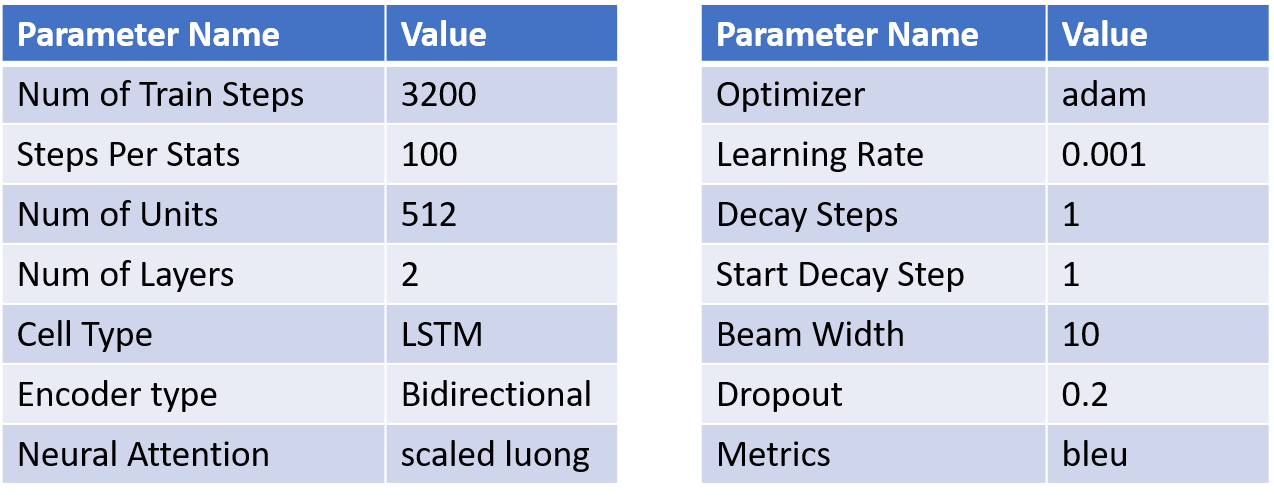
\includegraphics[scale=.7]{training_parameter}
\end{center}
\end{figure}
{\let\clearpage\relax \chapter {Result}}
\noindent Following are some response derived after training on full dataset with 34MB of training text with 225000+225000 utterance. The initial test result produced moderately coherent sentences. The following responses were generated after inference from trained model. In inference, trained model produced 10-30 candidate response for each input. Hence, the following examples are most suited from 10-30 candidate responses during inference.  
\begin{figure}[H]
\begin{center}
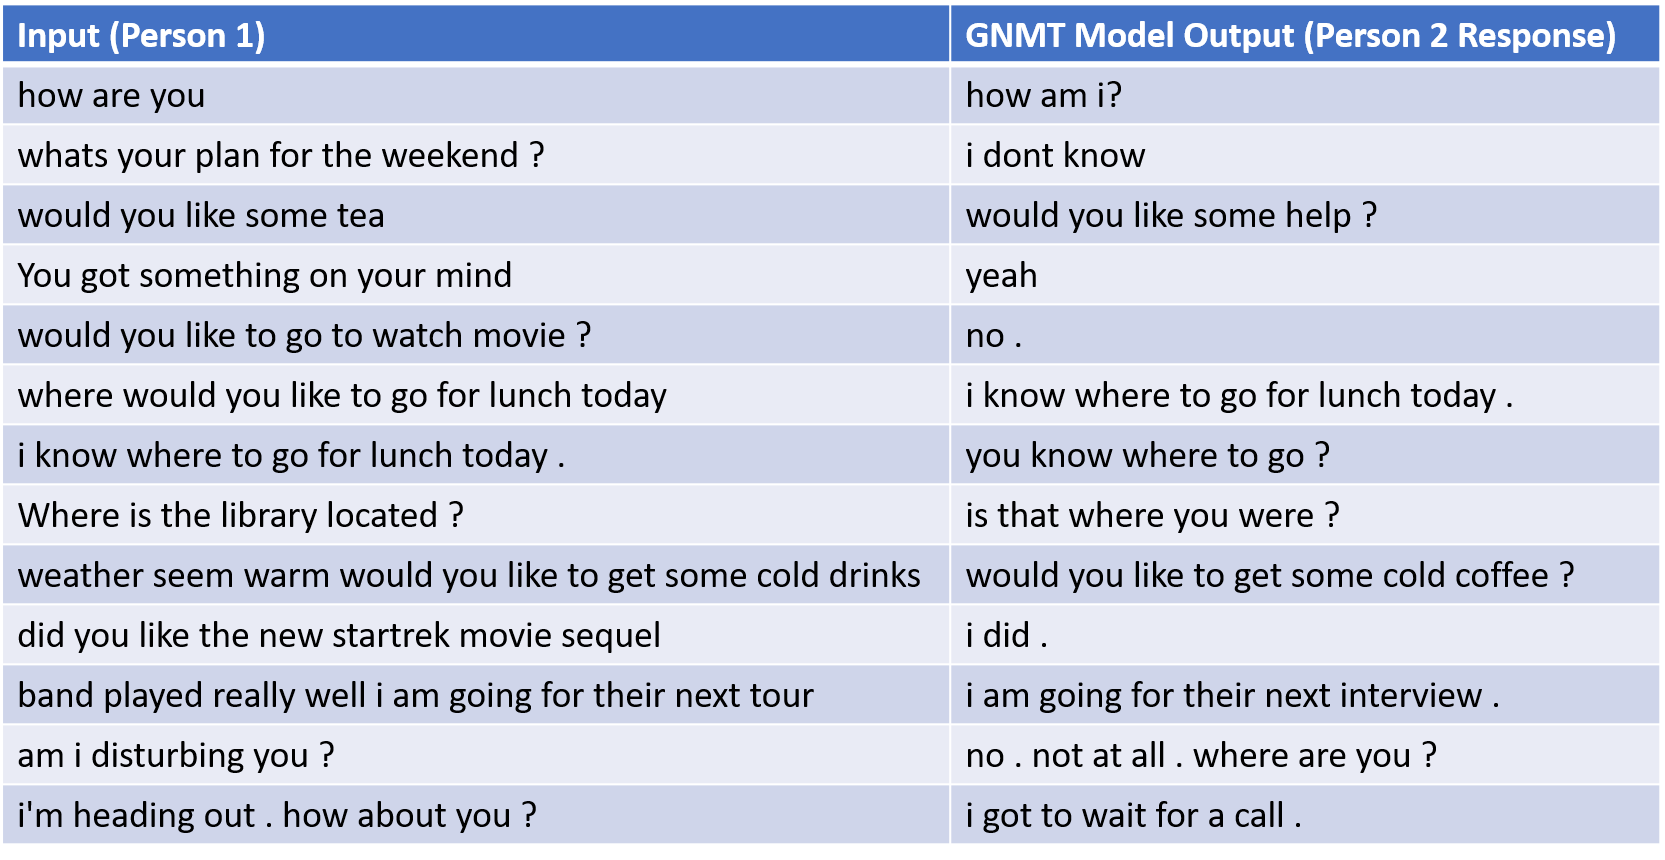
\includegraphics[scale=.6]{chat_gen}
\end{center}
\end{figure}
Following are the Perplexity and Bleu for test and development dataset
\begin{center}
\begin{table}[H]
\begin{center}
\caption{Evaluation}
\bigskip
\scalebox{1.5}{
\begin{tabular}{|l|l|l|}
\hline
Dataset & Perplexity & Bleu \\
\hline
eval dev & 50.76 & 10.1\\
eval test & 46.82 & 10.6\\
\hline
\end{tabular}}
\end{center}
\end{table}
\end{center}
{\let\clearpage\relax \chapter {Graphical Interface (GUI)}}
Desktop Graphical Interface (GUI) was developed using Python and PyQT module. On left top side, the chat response and history is shown, and on the right textarea, all possible response of input text was shown. As during chat model training, number of output or translation was around 30, more than one possible response is shown. On the left, one response of input text was randomly chosen from resultant responses generated after interference.   
\begin{figure}[H]
\begin{center}
\caption{Graphical Interface of Intelligent Chatbot}
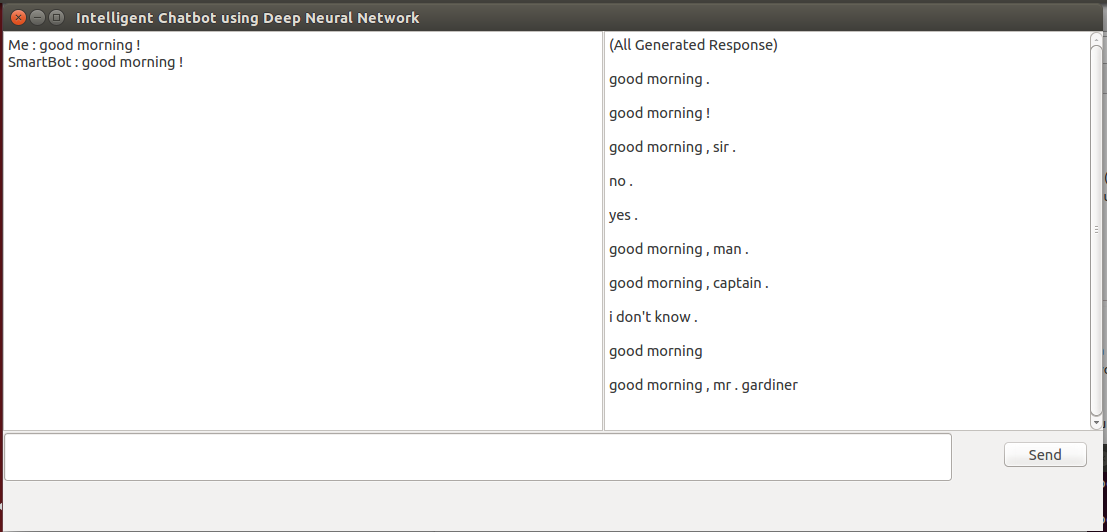
\includegraphics[scale=.4]{chat_gui}
\end{center}
\end{figure}
{\let\clearpage\relax \chapter {Challenges}}
\noindent The challenge in developing chatbot or dialogue generator lies in developing coherent dialogue generation system. As the model used in this experiment is for machine translation, the dialogue generation is treated as translation problem, where history of earlier conversations are not taken into account. Hence, the model can be limited in performance regarding long conversation.\\\\
Also, training is a long process which demands higher processing power and configured computing machine. Another problem is finding right hyper parameters to optimize the translation module for chat bot or dialogue generation system.\\\\
There are multiple chatbots developed using GNMT or Seq2Seq module. GNMT is a rather self-contained with Bi-directional LSTM cells, Neural Attention mechanism and Beam search techniques. Most of this features improve dialogue generation as well as machine translation. Bi-directional LSTM cells with attention mechanism seems to produce better output. Seq2Seq module also has some of the advanced features of GNMT. Nevertheless, developing chatbot algorithm from scratch by building RNN, bidirectional LSTM and neural attention techniques would be better suited option as GNMT is primarily for machine translation. But, this will require multiple trial and error before reaching optimal performance for the comprehensive chatbot module and hence is better suited as research problem.\\\\
After training, chatbot produced results with moderate relevancy. But many of the output were repeative and generic. Also, due to lack of real-life quality data the chatbot performed somehow below optimum for imitating human interaction. Also, many utterance was discarded due to longer length or discrepancy. And, number of training utterance was much less than required and test and development dataset was quite larger in comparison which might have caused the model to under-perform. Also, as data was limited, longer period of training may not have suited the dialogue generation problem.\\\\

{\let\clearpage\relax \chapter {Discussion}}
\noindent Development of dialogue agent using Neural Machine Translation(NMT) is widely practiced. Some other approaches use only Sequence to Sequence modeling. Many people also use their own Sequence to Sequence module. But, due to their lack complexity they fail to perform well. However, with more time and effort building a more comprehensive dialogue generation unit could solve dialogue generation problem is specifically better. Hence, Sequence to Sequence module with encoder-decoder architecture built on bi directional LSTM cells and Neural attention mechanism,Beam Search could be a more preferable task.\\\\
Apart from algorithm improvement, performance could be further optimized if better datasets were available. Before using Cornell Movie Dataset, I have experimented with other datasets and preprocessed and trained them on the GNMT module. But, due to lack of data quality, they were later discarded from training. Also, the datasets available used here are movie subtitles, which hardly mimics real human interaction. More realistic and high quality real life conversational data could further emulate the need and personality of the user. For future training, even personal chat history can be incorporated to give intelligent chatbot some personality.\\\\
The intelligent chatbot has produced moderate result. But, some of replies looks repetitive and lacks proper relevancy. This can be reduced with addition of more diverse and healthy data. Also, adding more length to original text could help improve responses and make them more relevant. A large proportion of data was lost due to choosing restrictive length where utterance more than 100 length was discarded but later full length text was adopted. This might have caused redundancy in training process. Also, repeated utterance by same character was eliminated and only last utterance by repeated speaker was kept, which further reduced data size. Therefore more data with optimum sequence length can help build more intelligent chatbot.\\\\

{\let\clearpage\relax \chapter {Future Work}}
\noindent The chatbot developed using Google's Neural Machine Translation Model(GNMT) can be further improved with more robust, high quality real-life conversational datasets which could better emulate human interaction. Also, hyper-parameters of the GNMT model can be further fine-tuned and optimized for performance enhancement. Based on available opportunity to further advance the project, Deep Reinforcement Learning(RL) can be applied that could significantly improve performance as shown empirically in Dufarsky's paper. Reinforcement Learning algorithm can be applied after the initial training using Google's Neural Machine Translation.\\\\

{\let\clearpage\relax \chapter {Conclusion}}
\noindent The training on Cornell Movie Subtitle corpus produced result which needs further improvement and more attention and speculation on training parameters. Adding more quality data will further improve performance. Also, the training model should be trained with other hyper-parameters and different dataset for further experimentation. This was an attempt to experiment with Deep Neural Network for dialogue generation inorder to develop intelligent chatbot. 
\begin{thebibliography}{}
\bibitem{jurafskyRL} 
Li J, Monroe W, Ritter A, Galley M, Gao J, Jurafsky D.
\textit{Deep reinforcement learning for dialogue generation.} 
arXiv preprint arXiv:1606.01541. 2016 Jun 5.

\bibitem{nmt} 
\textit{Google's Neural machine translation(NMT)} 
\url{https://github.com/tensorflow/nmt}

\bibitem{seq2seqtutorial} 
\textit{Neural Machine Translation (seq2seq) Tutorial} 
\url{https://www.tensorflow.org/tutorials/seq2seq}

\bibitem{seq2seq} 
\textit{seq2seq Github Repository} 
\url{https://github.com/google/seq2seq}


\bibitem{seq2seqgoogle} 
\textit{Google's seq2seq} 
\url{https://google.github.io/seq2seq/}

\bibitem{CornellMovieDialogs} 
\textit{Cornell Movie Dialogs Corpus}
\url{http://www.cs.cornell.edu/~cristian/Cornell_Movie-Dialogs_Corpus.html}\\\\

\end{thebibliography}
\newpage
{\let\clearpage\relax \chapter {References}}
\begin{enumerate}[align=left, rightmargin=\dimexpr\linewidth-14cm-\leftmargin\relax]
\item \url{https://medium.com/swlh/chatbots-of-the-future-86b5bf762bb4}
\item \burl{https://chatbotsmagazine.com/to-build-a-successful-chatbot-ask-these-5-questions-b7fe3776c74c}
\item \url{https://labs.bawi.io/creating-a-conversational-chatbot-using-wit-ai-6eba3c625f4f}
\item \url{https://www.ipsoft.com/2017/11/20/when-chatbots-fail-virtual-agents-step-in/}
\item \url{https://isaacchanghau.github.io/2017/08/02/Seq2Seq-Learning-and-Neural-Conversational-Model/}
\item \url{https://chatbot.fail/}
\item \url{https://www.altoros.com/blog/text-prediction-with-tensorflow-and-long-short-term-memory-in-six-steps/}
%\item \url{}
\item \url{https://medium.com/the-mission/11-best-uses-of-chatbots-right-now-1c27764b7e62}
\item \url{https://www.marutitech.com/7-reasons-why-business-needs-chatbot/}
\item \url{https://chatbotsmagazine.com/how-to-develop-a-chatbot-from-scratch-62bed1adab8c}
\item \url{https://www.marutitech.com/complete-guide-bot-frameworks/}
\item \url{https://en.wikipedia.org/wiki/Long_short-term_memory}\\\\
\end{enumerate}
\newpage
{\let\clearpage\relax \chapter {Image Credits}}
\begin{enumerate}[align=left, rightmargin=\dimexpr\linewidth-14cm-\leftmargin\relax]
\item \url{https://regmedia.co.uk/2017/09/21/chatbot.jpg?x=442&y=293&crop=1}
\item \url{https://cognitiveseo.com/blog/wp-content/uploads/2017/06/Is-Chatbot-Marketing-the-future-1024x512.jpg}
\item \url{http://nyintl.net/site/wp-content/uploads/2018/01/robot-customer-service.png}
\item \url{https://cdn.zmescience.com/wp-content/uploads/2015/06/robot.jpg}
\item \url{http://www.netalogue.com/wp-content/uploads/2017/03/chatbot-880x541.png}
\item \url{https://betanews.com/wp-content/uploads/2017/08/chatbot-e1501792996887.jpg}
\item \url{https://www.adityathakker.com/wp-content/uploads/2017/05/Facebook-Messenger-ChatBot-tutorial.jpg}
\item \url{https://cdn-images-1.medium.com/max/1200/1*FYFI4jbAUMqbXxlo6V_lBA.png}
\item \url{http://sunnyapps.co/assets/images/temp/sunnyapps-chatbots-about.png}
\item \url{https://www.liveworld.com/wp-content/uploads/2017/07/Chatbots-in-customer-service_cropped.png}
\item \url{https://cdn-images-1.medium.com/max/1200/1*fNPqCg4vBiCQS1-nFs7gYA.jpeg}
\item \url{https://cdn-images-1.medium.com/max/1600/0*LyfY3Mow9eCYlj7o.}
\item \url{https://www.dailydot.com/wp-content/uploads/0da/df/dominos.jpg}
\item \url{https://bot-hub.com/media/print_screen/Yahoo-Weather/yahooweather__4.jpeg}
\item \url{https://chatfuel.com/images2/og_chatfuel.jpg}
\item \url{https://4.bp.blogspot.com/-UWs8Wger9LQ/WQ8Uh05oMzI/AAAAAAAABrc/oFhlMOasZZIxjDZOxmXGEJLBIfTd2VETACLcB/s1600/bottr-for-blogger.jpg}
\item \url{http://static.hackingrevenue.com.s3.amazonaws.com/2016/08/motionai_0.png}
\item \url{https://botlist.co/system/BotList/Bot/logos/000/000/627/medium/recast_ai.png}
\item \url{https://techcrunch.com/wp-content/uploads/2016/09/api.jpg}
\item \url{http://www.dieproduktmacher.com/wp-content/uploads/2017/08/lex-vs-api.png}
\item \url{http://bodhiinfo.com/blog/wp-content/uploads/2016/09/google-apiai.jpg}
\item \url{https://cdn-images-1.medium.com/max/860/1*QoCscxdXl2mkWqL7mGfALA.png}
\end{enumerate}
\end{document}

